\documentclass{article}
\usepackage{pdflscape}
\usepackage[margin=1in]{geometry}
\usepackage{verbatim}
\usepackage{graphicx, float}
\usepackage{makecell}
\usepackage{amsmath}
\usepackage{amsfonts}
\usepackage{amssymb}
\usepackage{bookmark}
\usepackage{enumitem}
\usepackage{pdfpages}
\usepackage{listings}
\usepackage{listings-ext}
\usepackage{hyperref}


\author{Astrid Augusta Yu}
\title{CPE 233 Lab \#6 -- Complete ISA RISC-V MCU}
\date{\today}

\DeclareMathOperator\bit{bit}
\DeclareMathOperator\byte{byte}
\DeclareMathOperator\word{word}

\begin{document}
\maketitle

\tableofcontents

\section{Questions}

\begin{enumerate}
    \item\textbf{Briefly but completely explain why, in general, why is it important to keep your ISRs as short as possible.  }

    It is important to keep ISRs short because that way, the program will be able to respond to the interrupt faster. If the ISR is too long then it might miss another interrupt while processing the first.

    \item\textbf{We often consider the ISR code as having a “higher priority” than the non-interrupt code. Briefly but fully explain this concept.  }

    In the event of an interrupt, the ISR code will be executed before any other code. Thus, it has higher priority because it is executed first.

    \item\textbf{If you were not able to use a LUT for this experiment, briefly but completely describe the program you would need to write in order to translate a given BCD number into its 7-segment display equivalent.  }

    You would essentially be writing the list/LUT in code. One way to do it would be to perform a linear search, where you check the BCD value against 0, then 1, then 2, and so on, until 9. Another implementation could potentially execute in a shorter amount of time: instead of doing a linear search, do a binary search (check $\geq 5$, if greater, check $\geq 7$, etc.). However, this would take a larger amount of program space. 

    \item\textbf{What is the minimum execution time of an ISR requires? This is the time from when the MCU switches to the interrupt state to when the processor begins executing the next intended instruction, which was scheduled to be executed before the interrupt processing started. Provide a concise answer with adequate description. Assume the interrupts return from the ISR in the disabled state.  }

    The smallest ISR possible is composed of a single MRET. The MCU is in the INTR state for 1 cycle. The MRET takes a LOAD and EX state to complete. Then, it returns to the next intended instruction. The minimum ISR execution time is thus 3 cycles.

    \item\textbf{As you know, part of the interrupt architecture includes the RISC-V MCU automatically masking the interrupts. This being the case, why then is there a need to keep the overall output pulse length of the interrupt relatively short?  }
    
    This is necessary because if the interrupt is unmasked while the pulse is still high, the interrupt will get triggered again.

    \item\textbf{Nested subroutines are quite common in assembly language programming. Accordingly, there is also the notion of nested interrupts? Briefly explain how you could allow nested interrupts to occur under program control on the RISC-V MCU.  }

    The CSR would need to be modified to support multiple interrupts. This would be done by 

    \item\textbf{In theory, how deep could you nest interrupts on the RISC-V MCU? Briefly but concisely explain. }
    
    You can nest interrupts infinitely deep by unmasking interrupts during the ISR. This would have the potential consequence of the MCU falling into an infinite loop where it keeps getting interupted during its ISR. 

    \item\textbf{Write some RISC-V OTTER assembly code that would effectively implement a firmware debounce for a given button. For this problem, assume the button you’re debouncing is associated with the LSB of buttons addressed by port 0x1100\_8004. Make sure to fully describe your code with instruction comments and header comments. Also include a flowchart that models your code.  }
    
    \lstinputlisting{q8.asm}

    See next page for flowchart.

    \includepdf[pages=-]{q8.pdf}

    \item\textbf{You wrote assembly code for this experiment. Briefly but completely explain whether this code was software, firmware, or wankware.  }

    The assembly code written was both software and firmware. It is software because it is not a physical module, but a series of instructions that is executed by the MCU. It is firmware because it interacts directly with the hardware without much abstraction. 

    \item\textbf{State whether the RISC-V MCU is a RISC or CISC processor. Support your statement with at least three characteristics regarding those two types of computer architectures.  }
    
    The RISC-V MCU is a RISC processor. All of its instructions execute in either 2 or 3 cycles; instructions are relatively simple in terms of function; and there are 32 registers in the register files, a fairly large number compared to the 8 general-purpose registers in x86, a CISC architecture.

    \item\textbf{Although they sort of sound the same, briefly describe the difference between receiving an interrupt and acting on an interrupt.  }
    
    Receiving an interrupt is when the MCU sees a high INTR pin and enters an interrupt cycle. Acting on an interupt is when the MCU actually runs the code in the ISR. 

\end{enumerate}

\pagebreak
\section{Programming Assignment}
\lstinputlisting{pg.asm}

\pagebreak

\section{Hardware Assignment}

\textbf{You must modify the RISC-V MCU such that the mret instruction automatically unmasks the interrupts. Describe which RISC-V OTTER modules need to change and what changes those modules requires. Show the code you change as part of this solution. This is one of those problems that requires only a few minutes after you think about it for an hour. You’re going to need to look at the CSR module to do this problem.}

This can be solved by creating a new signal between the CU\_DCDR and CSR called set\_mie. In the CU\_DCDR file, it will raise set\_mie whenever the processor is executing a MRET instruction:

\begin{lstlisting}[language=Verilog]                
module CU_DCDR(
    input br_eq, 
    input br_lt, 
    input br_ltu,
    input int_taken,

    input [6:0] opcode,   //-  ir[6:0]
    input [6:0] func7,    //-  ir[31:25]
    input [2:0] func3,    //-  ir[14:12] 

    output logic [3:0] alu_fun,
    output logic [2:0] pcSource,
    output logic alu_srcA,
    output logic [1:0] alu_srcB, 
    output logic [1:0] rf_wr_sel

>   output logic set_mie
    );

    ...
    always_comb begin 
>       set_mie = 0

        ...
            
            OP_INT: if (func3[0]) begin  // csrrw
                rf_wr_sel = 2'd1;  // csr_reg
                pcSource = 3'd0;  // next
            end else begin  // mret
                pcSource = 3'd5;  // mepc
>               set_mie = 1;
            end
\end{lstlisting}

The CSR file will be modified to raise CSR\_MIE every whenever set\_mie is high.

\begin{lstlisting}[language=Verilog]
module CSR(
    input CLK,
    input RST,
    input INT_TAKEN,           
    input [11:0] ADDR,
    input [31:0] PC,
    input [31:0] WD,
    input WR_EN,
>   input set_mie,     // Add an input signal to CSR, raised during a MRET
    output logic [31:0] RD,
    output logic [31:0] CSR_MEPC=0,  //- return from interrupt addr
    output logic [31:0] CSR_MTVEC=0, //- interrupt vector address  
    output logic CSR_MIE = 0      ); //- interrupt enable register

    // ...

    always_ff @(posedge CLK) begin
        // ...
        if (WR_EN) case(ADDR)
            MTVEC: CSR_MTVEC <= WD;    //- vector addr
            MEPC:  CSR_MEPC  <= WD;    //- return addr
            MIE:   CSR_MIE   <= WD[0]; //- interrupt enable
>       endcase else if (set_mie)
>           CSR_MIE <= 1                // Set MIE during MRET
>       end
\end{lstlisting}

The MRET signal is connected to the CU\_DCDR. It is 1 whenever a MRET is being executed, but 0 every time else.

\pagebreak

\section{Assembly Code}
\lstinputlisting{otter-e8.asm}
\section{Flowchart}

Flowchart begins on next page.
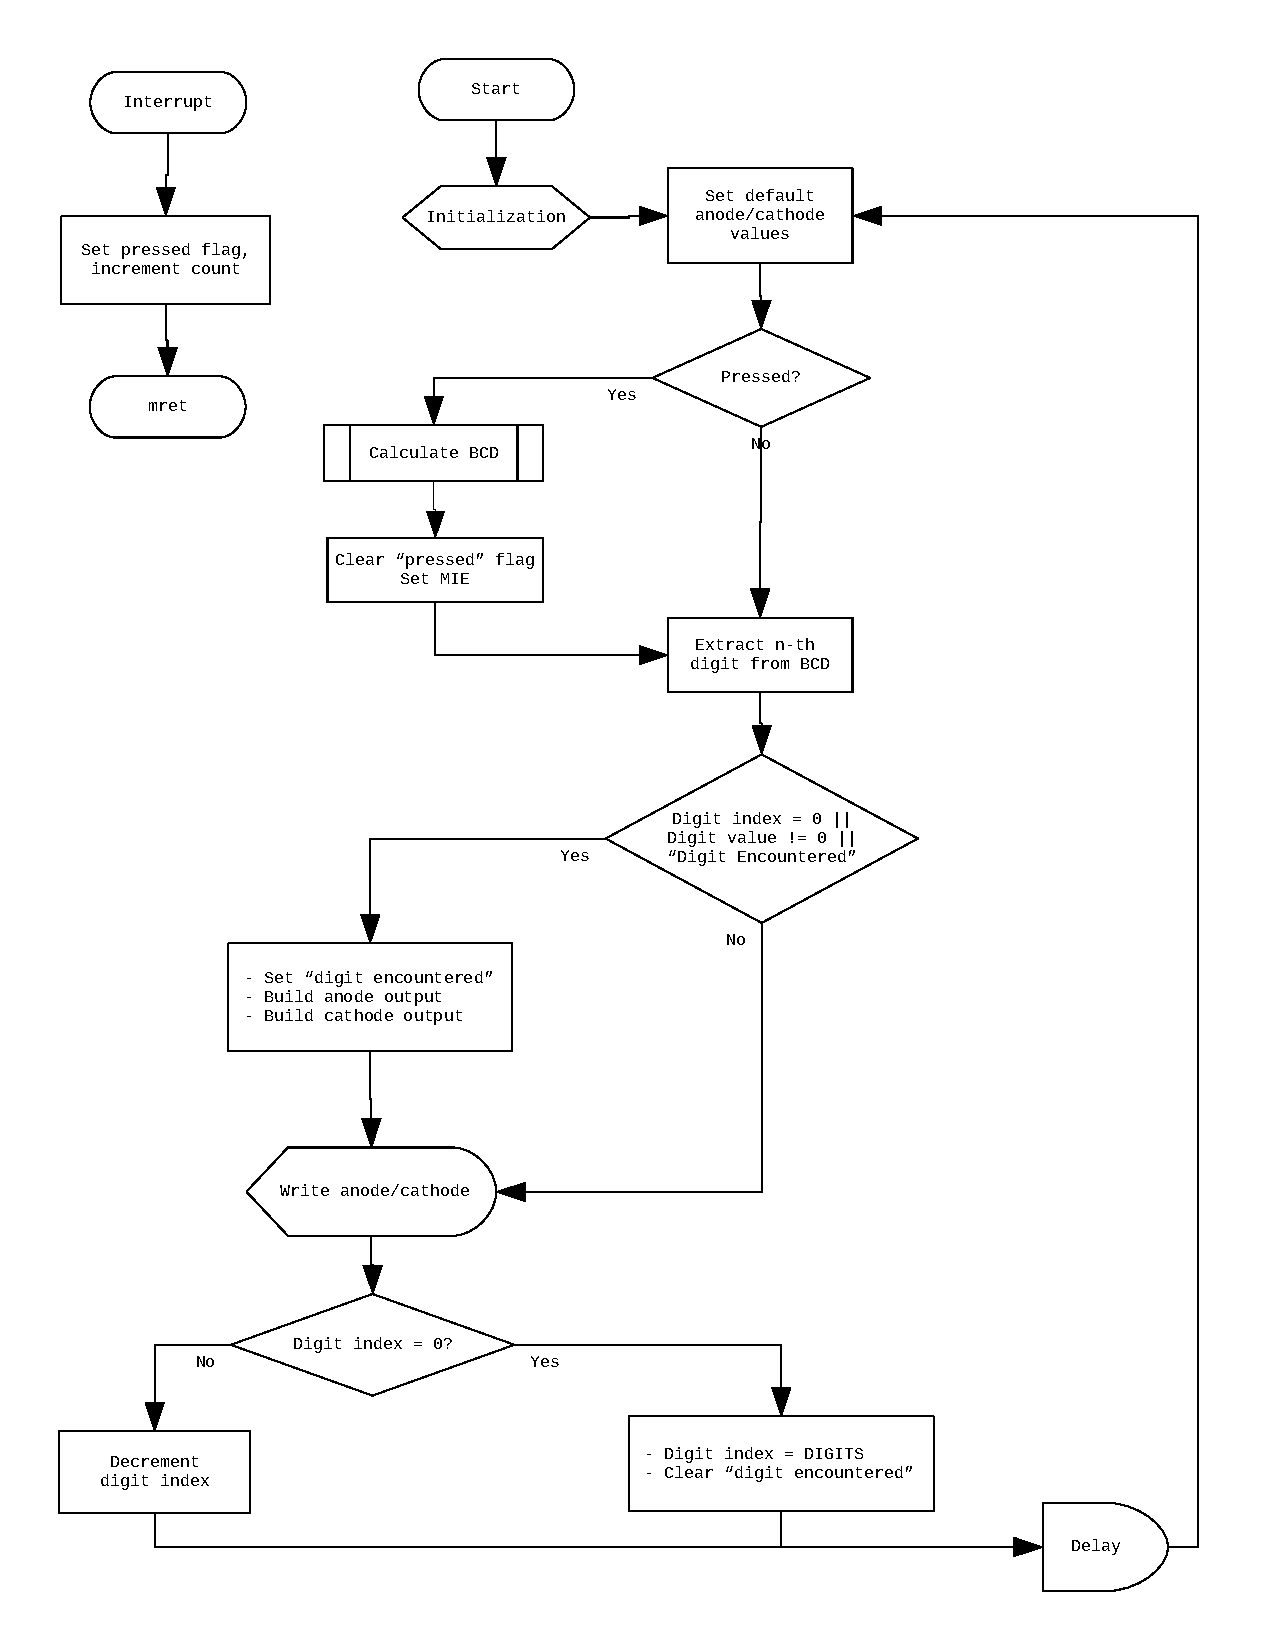
\includepdf[pages=-]{flowchart.pdf}

\begin{landscape}
\section{Hardware Schematic}
\centering
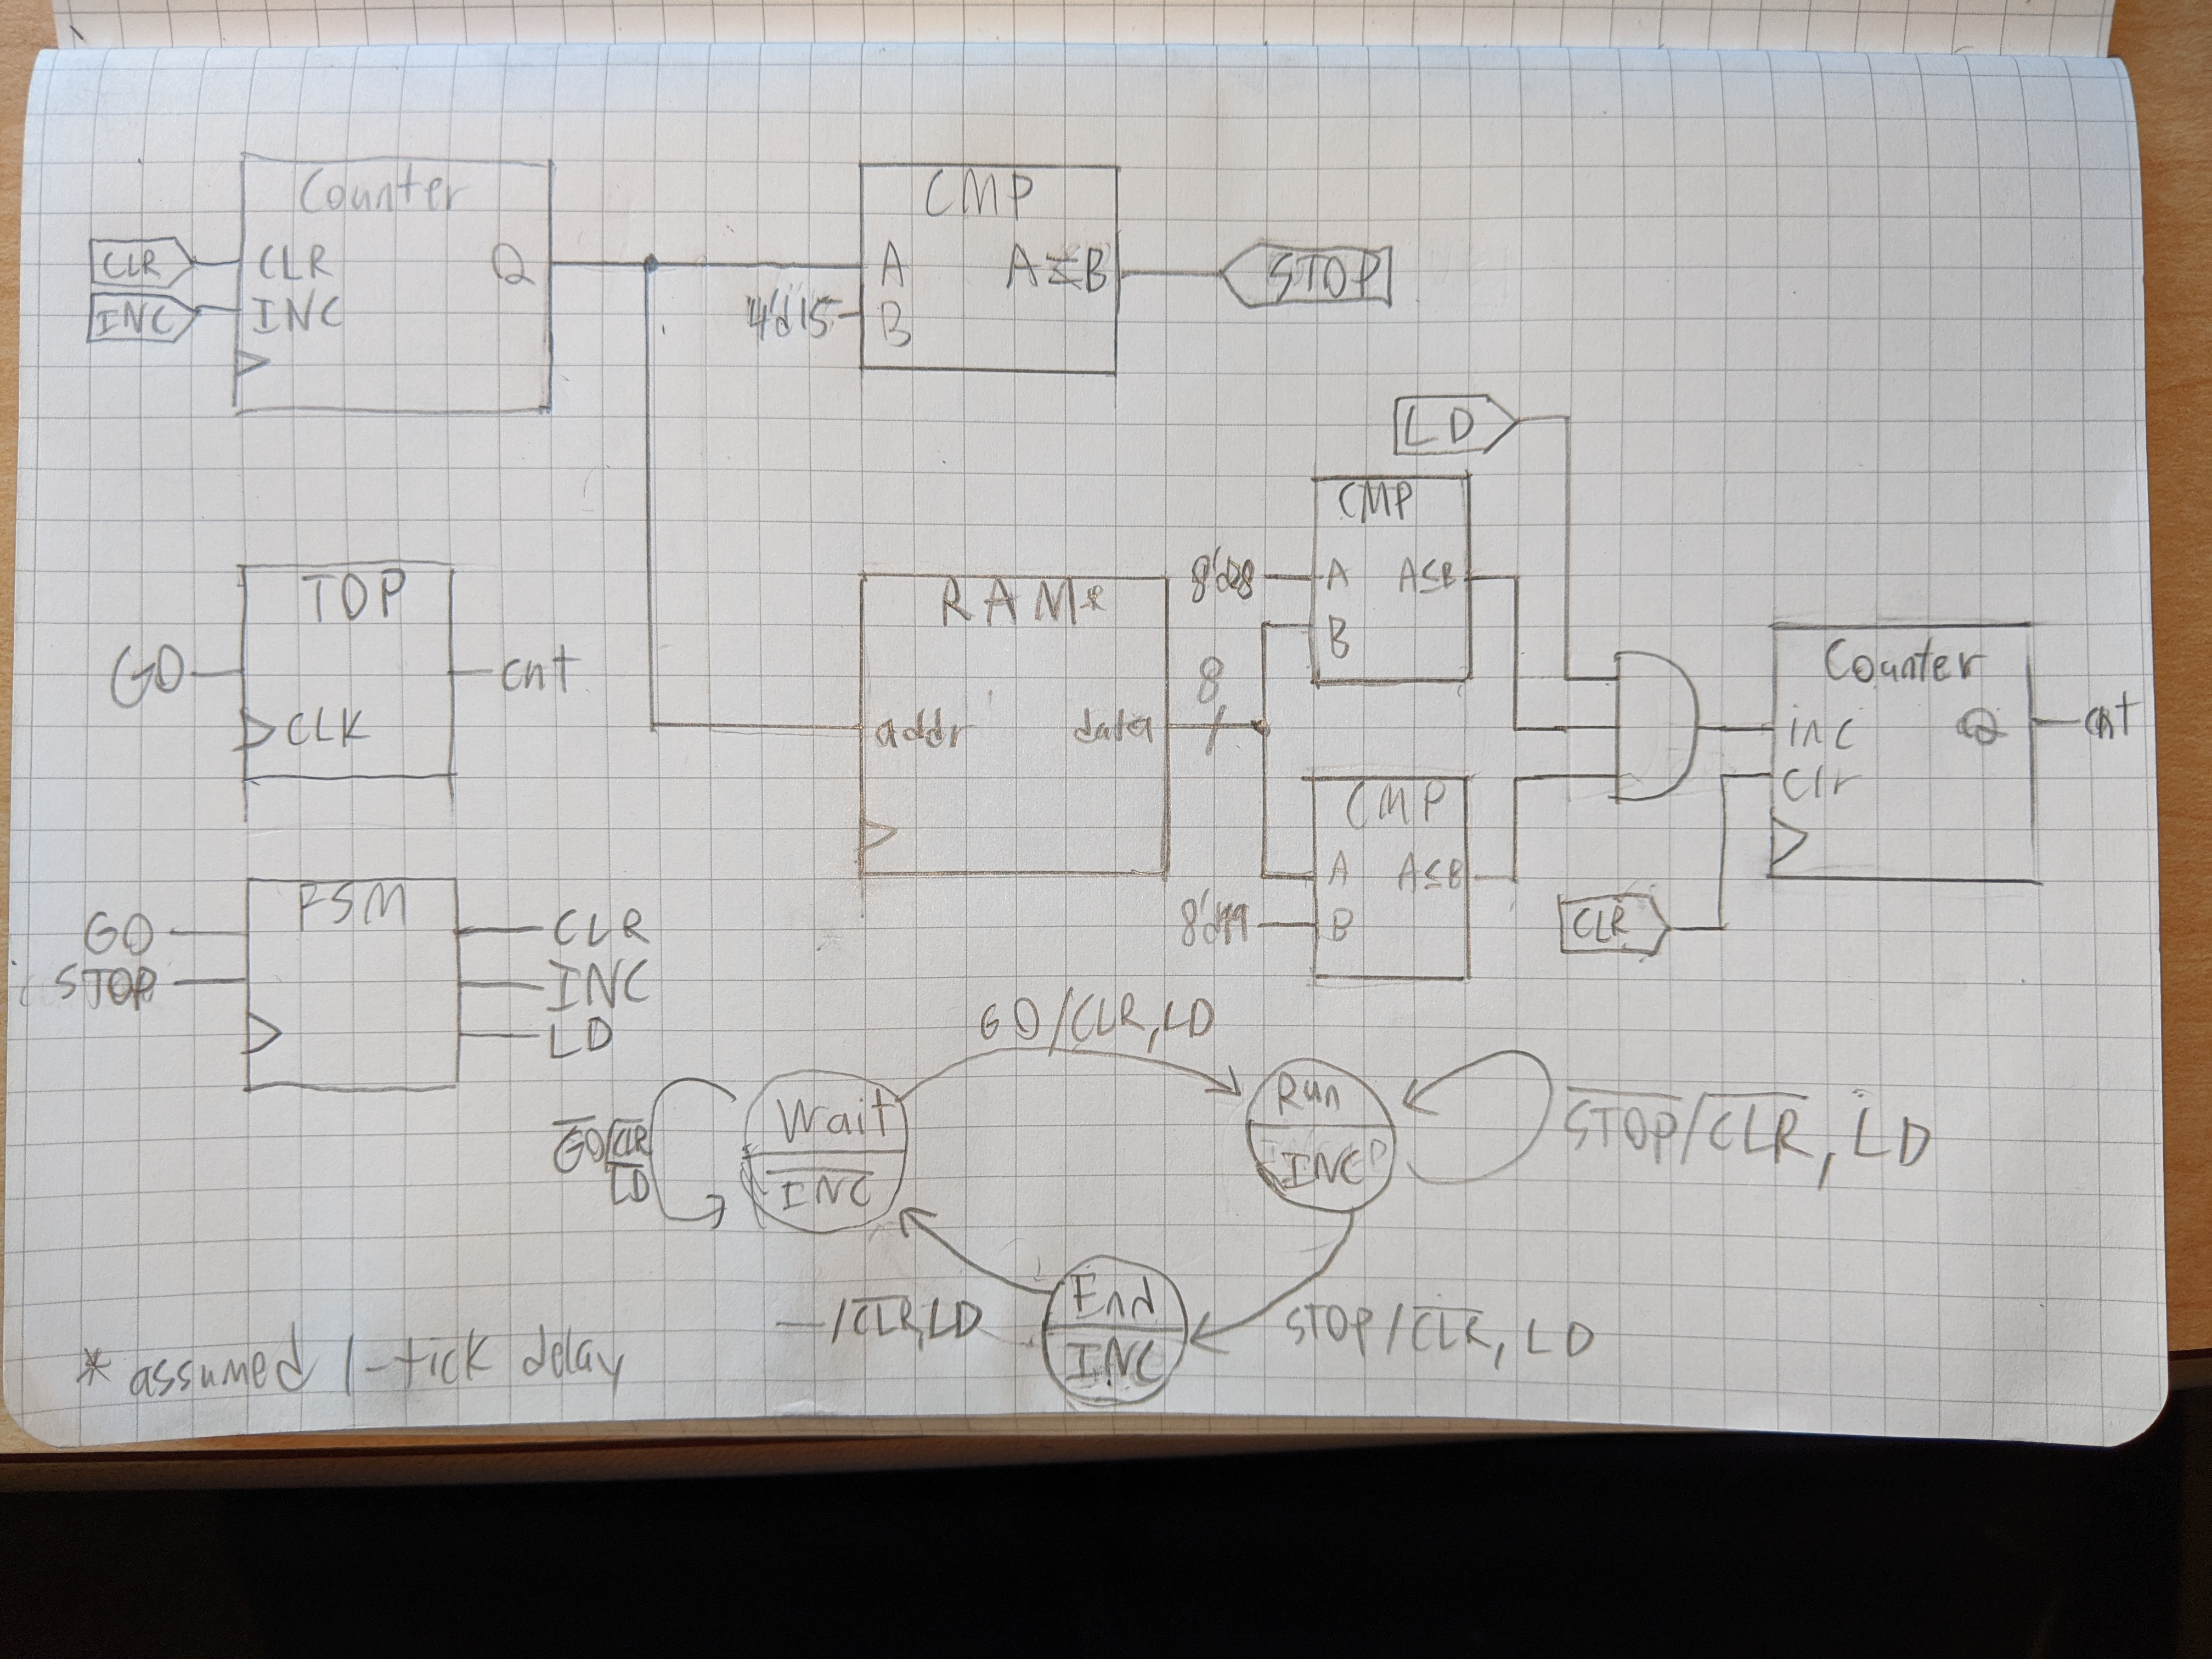
\includegraphics[width=0.92\linewidth]{hw.jpg}
\end{landscape}

\end{document}
